\section{Empirical Evaluation}
\label{sec:eval}


We conducted two empirical studies using two open-source applications 
and one IBM proprietary application. In the first study, we evaluated the
effectiveness of our technique in covering rules, whereas in the second study
we compared our technique with a naive technique. After describing the experimental setup,
we present the results of the two studies.

\subsection{Experimental Setup}

\subsubsection{Implementation}
\label{sec:impl}


\begin{table}[t]
\caption{Subjects used in our empirical studies.}
\centering
{\scriptsize
\tabcolsep=3pt
\begin{tabular}{|l|l|r|r|r|r|}
\hline
\multicolumn{1}{|c|}{Subject} & \multicolumn{1}{|c|}{URL} & \multicolumn{1}{|c|}{Entities} & \multicolumn{1}{|c|}{Operations} & \multicolumn{1}{|c|}{Rules} & \multicolumn{1}{|c|}{Rule parts} \\
\hline \hline
Cebu-pacific & www.cebupacificair.com 		& 8  & 10 &  	 & 31 \\
jBilling 		 & www.jbilling.com 					& 10 & 10 &   	 & 26 \\
App 				 & \multicolumn{1}{|c|}{---}	& 12 & 13 &     & 20 \\
\hline \hline
\textbf{Total} & 													& 	 & 33 &     & 77 \\
\hline
\end{tabular}
}
\label{tab:subjects}
\end{table}

\subsubsection{Subjects and Rules}

We used two open-source applications and one IBM proprietary application, listed
in Table~\ref{tab:subjects}, as experimental subjects. Due to confidentiality reasons,
we refer to the proprietary application as \subject{App}. \subject{Cebu-pacific} is
an airlines application, \subject{jBilling} is an enterprise billing application,
and \subject{App} is a telecom application. Column~2 shows URL of each subject.
Columns~3--6 show additional details such as number of entities, operations,
and rules. For each subject, we identified a module that is likely to have large
number of interesting rules with respect to test data, and modeled those modules using our tool. In particular,
we used \textit{ticket cancellation} and \textit{generate invoice} modules for \subject{Cebu-pacific} and 
\subject{jBilling}, respectively. Overall, we modeled $33$ operations with $XX$ rules and
$77$ rule parts.

\subsubsection{Method}


\subsection{Coverage of Business Rules}

\begin{figure}[t]
\centering
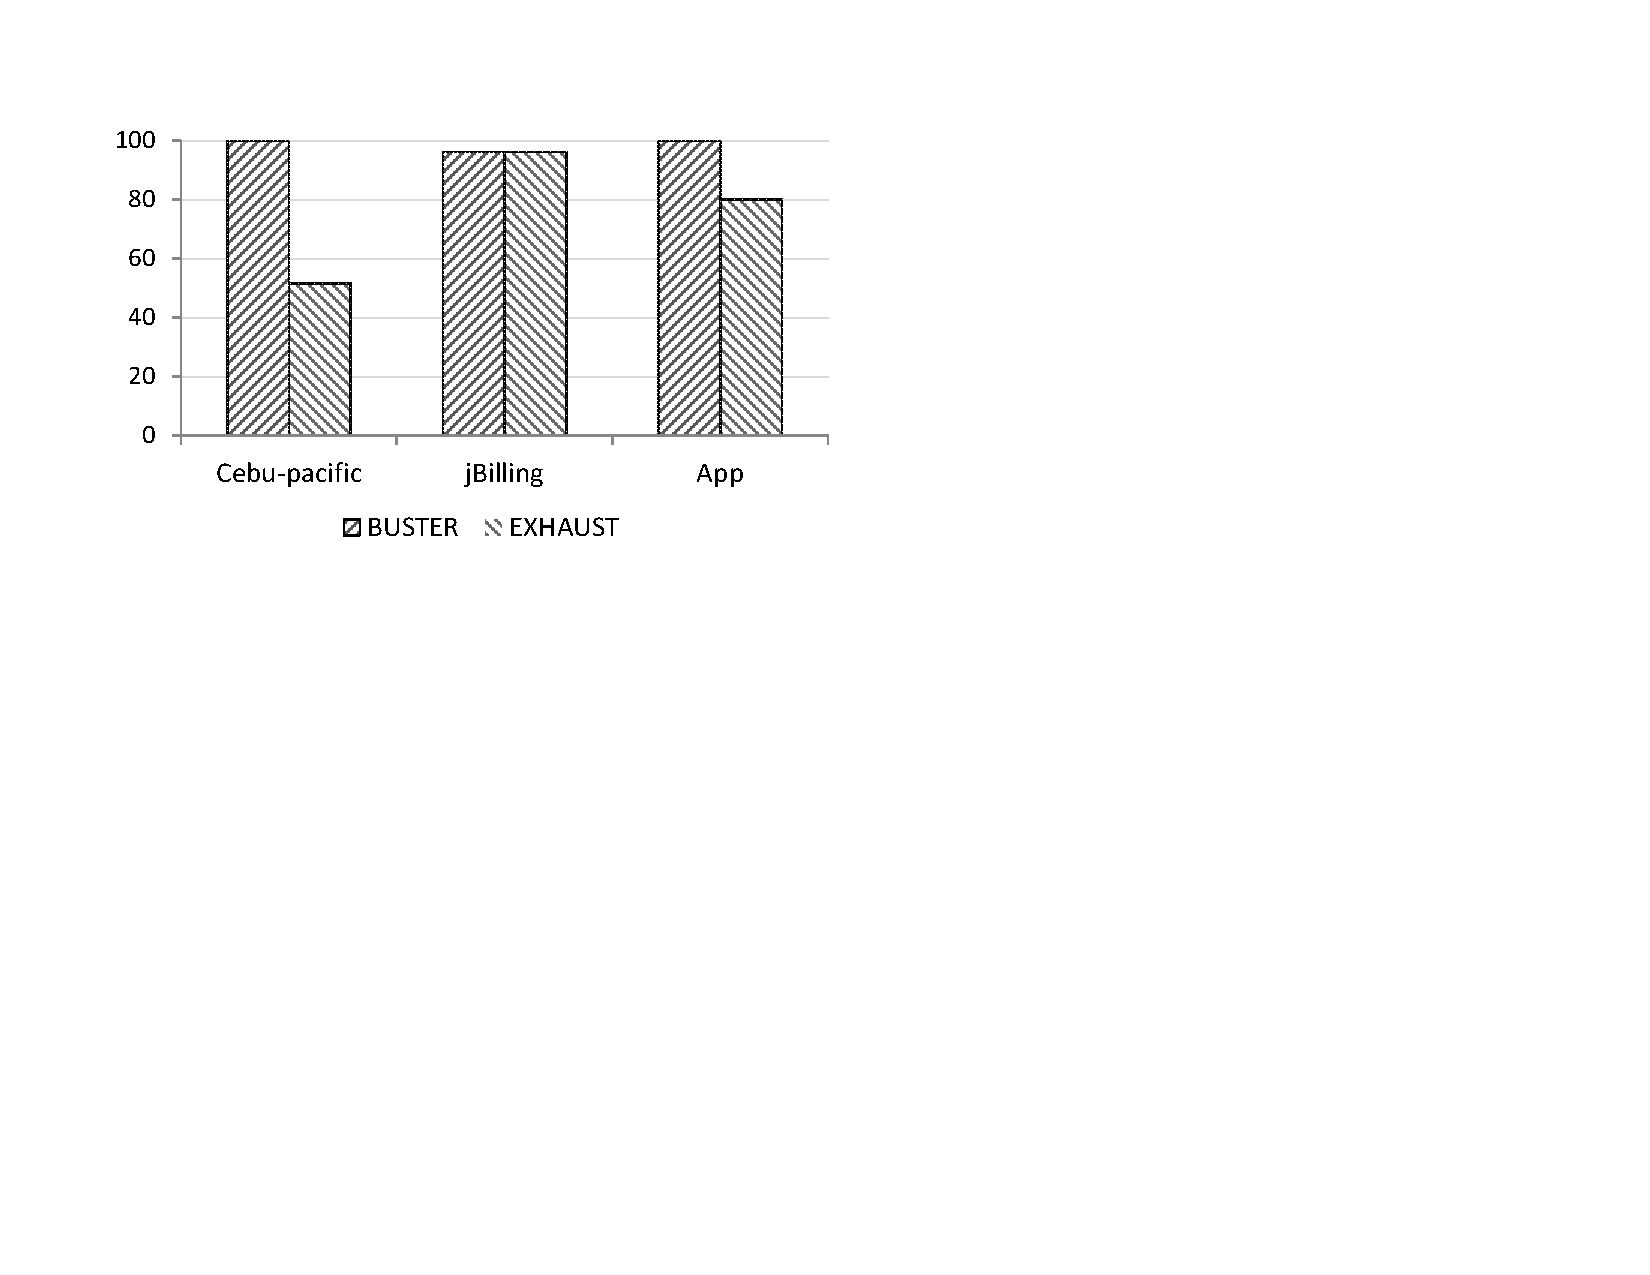
\includegraphics[width=\columnwidth, clip, trim = 18mm 120mm 140mm
  18mm]{Figs/Study-1.pdf}
\caption{Effectiveness of the two techniques in covering business rules.}
\label{fig:effectiveness}
\end{figure}

Figure~\ref{fig:effectiveness} shows the results for all three subjects. 
In the figure, x axis shows subjects, whereas y axis shows the percentage of rule parts
covered by each technique. For example, for \subject{Cebu-pacific},
our technique generated tests for all $31$ rule parts, whereas the naive technique was able
to generate tests only for $16$ rule parts. Overall, our results show 
that our technique handled $99$\% of all rule parts, whereas the naive technique
could handle $74$\% of all rule parts. Apart from higher effectiveness compared
to the naive technique, the next subsection shows that our technique is more efficient
as well.

In our inspection, we identify that the rules that were not covered by naive technique
are complex and require carefully crafted sequences. In particular, naive technique
was able to perform well in the scenarios where there exist only a few operations
that modify entities, which is the case with \subject{jBilling}. Instead, it could not
perform well for other two subjects where there exist many operations that modify
entities. Both ours and naive technique could not cover one rule part in \subject{jBilling}
due to the limitation of underlying Choco constraint solver which was throwing 
out of memory error while solving the composed formula for that rule part. Overall,
our results show promising benefits of our technique in effectively generating
tests for covering business rules.

\subsection{Additional Statistics}


\begin{table}[t]
\caption{Additional statistics of exploration.}
\centering
{\scriptsize
\tabcolsep=3pt
\begin{tabular}{|l|r|r|r|r|r|r|r|r|}
\hline
& \multicolumn{4}{|c|}{Sequence Length} & \multicolumn{4}{|c|}{\# of Sequences Explored} \\
\cline{2-9}
& \multicolumn{2}{|c|}{Ours} & \multicolumn{2}{|c|}{Naive} & \multicolumn{2}{|c|}{Ours} & \multicolumn{2}{|c|}{Naive}  \\
\cline{2-9}
\multicolumn{1}{|c|}{Subject} & \multicolumn{1}{|c|}{Max} & \multicolumn{1}{|c|}{Avg} & \multicolumn{1}{|c|}{Max} & \multicolumn{1}{|c|}{Avg} & \multicolumn{1}{|c|}{Max} & \multicolumn{1}{|c|}{Avg} & \multicolumn{1}{|c|}{Max} & \multicolumn{1}{|c|}{Avg} \\
\hline \hline
Cebu-pacific 	 &  7		& 5 &  9 &  5	 &  27 &  4	&  100 & 73 \\
jBilling		 	 &  6		& 3 &  6 &  3	 &  48 &  2	&  39  &  2 \\
App					 	 &  9		& 6 & 10 &  6	 &  51 &  5	& 100  & 46 \\
\hline
\end{tabular}
}
\label{tab:stats}
\end{table}

We next present data about the sequences that were produced by both ours and
the naive technique. Table~\ref{tab:stats} shows the data. Columns~2--5 show
the maximum and average length of sequences generated by both the techniques
across all rule parts. On the other hand, Columns~6--9 show the number of 
sequences explored by each technique across all rule parts. 

The results show that our technique is able to generates sequences of length $9$
for covering rule parts. Also, for a few rule parts, sequences generated by our technique are shorter
compared to the naive technique. Apart from the length of sequences, number
of explored sequences help show the efficiency of our technique. For example,
for \subject{Cebu-pacific}, our technique explored an average of $4$ sequences
(maximum of $27$), whereas the naive technique explored an average of $73$ sequences
per rule part. The results show that our technique is highly efficient showing
the effectiveness of our algorithm guided by the unsatisfiable core.
